\chapter{Design Consideration}
In this chapter the system will be designed with a top-down approach. First a use-case of the overall functionalities in the system is described, in order to give an overall view of what the system must be able to do. Furthermore ..  

\section{Use case design}
To give an overall view of what the system should be able to do, a UML use-case diagram is used to consider and describe the main functionalities and operators in the system, see \figref{fig:usecase}.

 \begin{figure}[H]
	\centering
	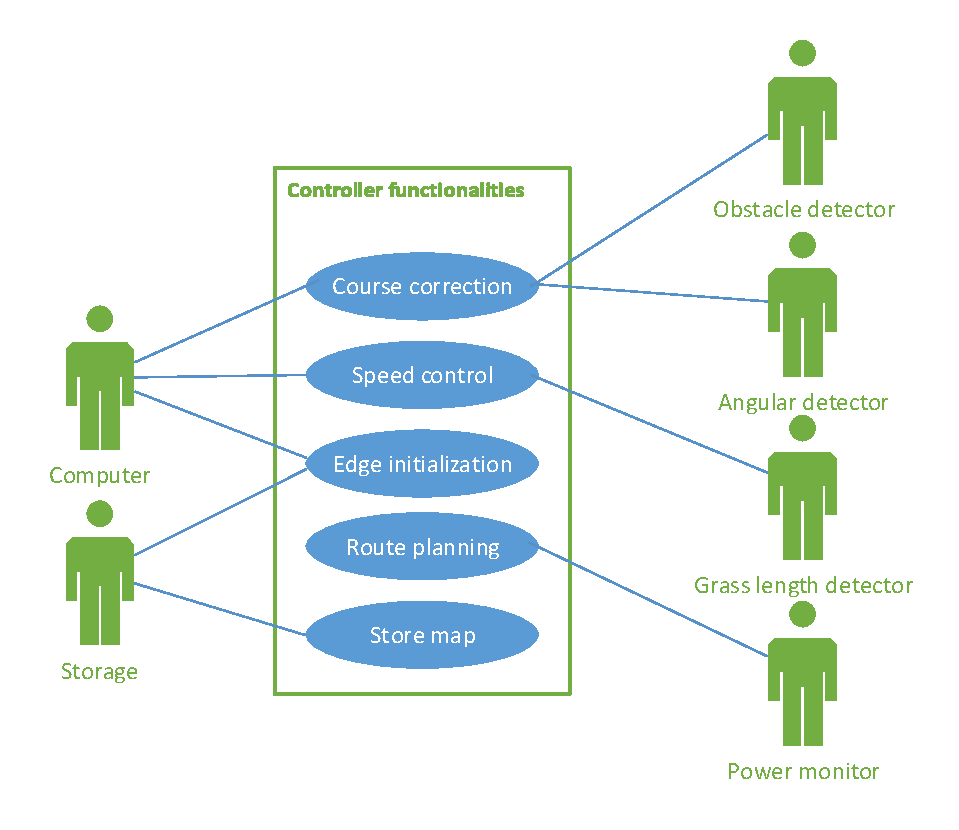
\includegraphics[scale=0.9]{figures/P5UseCase.pdf}
	\caption{Use-Case Diagram}
	\label{fig:usecase}
	\flushleft
\end{figure}

\noindent
The main purpose of the system is to automatically navigate in a specific area. In which area to navigate is set up by the \textit{Edge initialization} functionality, where the area is setup, by marking the edge of the area.\textit{Edge initialization} uses the \textit{Store map} functionality to store the information about the area, in storage. \\\\ 
The route to navigate after, in the specific area, is provided by the functionality \textit{Route planning}. \textit{Route planning} uses the information, about the specific area, that it gets from the storage, to plan the most optimal route in which to follow. Furthermore the \textit{Route planning} needs information about the systems power level to insure the \textit{Route planning} takes into consideration if the system needs charging and have to return to the charging station.\\\\
To insure the system is moving with a constant speed or a speed which is fitted to the height of the grass, detected with the \textit{Grass length detector}, a \textit{Speed control} functionality is necessary in the system.\\\\
The last functionality, \textit{Course correction} makes correction for the route, if something is standing in the way, which is detected by the \textit{Obstacle detector}, return the car to the charging station, if it starts to rain, which is detected by the \textit{Rain detector}, or if the system gets of the course, that is made by the \textit{Route planning} functionality.
The \textit{Course correction} sends the regulations about turns to the \textit{Speed control}, which will make the motors start to turn.\\\\
The course correction is the brain speed control is the muscles. 
Remember to put in the rain detector in the picture.
The GoT system input from the computer.
The slipping/not flat lawns and the angular sensor part.



 
 